%===================================== CHAP 5 =================================

\chapter{Test cases and results}

\subsection{Constant weight}

\begin{figure}[hbt!]
    \centering
    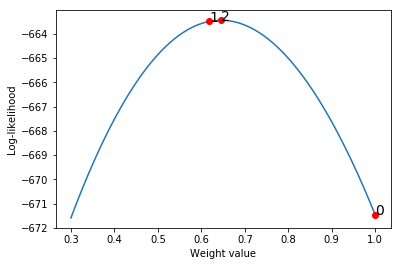
\includegraphics[scale=0.8]{Newton_method.png}
\end{figure}

Saturates at maximum after two iterations only. Output value corresponding to the plot was 0.645 for real weight equal to 0.7. This was for T equal to 1000.

\begin{itemize}
    \item Inferring constant weight using Newton method. Figure
    \item Inferring constant weight with Metropolis-Hastings
\end{itemize}

\subsection{Inferring dynamic weights}
Now the weights are let to vary. This makes the number of unknown parameters change from one to $T$. As described in section ??, as the number of data points is the same as the number of parameters, we need to take advantage of prior knowledge to infer the weights. This section presents the investigation of inferring dynamic weights using the Metropolis-Hastings algorithm.

For all test cases in this section we consider the case of having $T=10$. The weight corresponding to $t_{10}$ is not interesting, as no spikes are generated by it. Therefore there are 9 weights to infer. The true weights used in the spike simulations are set by specifying the weight at $t=t_1$ to be 0.7, $W_{t_1}^0 = 0.7$. The remaining weight trajectory is drawn as the weight of the previous time step plus the absolute value of a normal distributed parameter with zero mean and variance equal to $0.001$. This is a unrealistic big variance. In reality the number of time steps is much larger, and changing much slower. However, it is chosen this way to easily gain insight into the issue of inferring varying weights. \\

\textsc{Starting iterations from true weights}\\
For the first case the true weight trajectory is plotted in the following figure. 


\begin{figure}[hbt!]
    \centering
    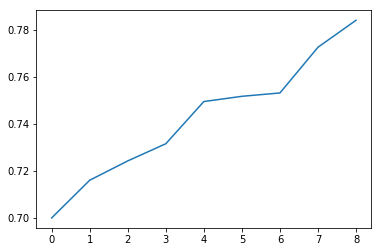
\includegraphics[scale=0.8]{Underlying.png}
\end{figure}

The following plot shows the normalized mean squared error when using different number of trials, starting the iterations from the correct weights. The variance used in the proposal and prior distribution is equal to $0.0001$. The number of iterations was 3000.

\begin{figure}[hbt!]
    \centering
    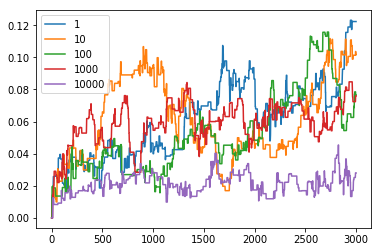
\includegraphics[scale=0.8]{MSE3.png}
\end{figure}

The same was done 100 times for each number of trials. The underlying weights were drawn new for each replicate. The following plot shows the mean of the MSE values at each iteration, with variance bars around it. 

\begin{figure}[hbt!]
    \centering
    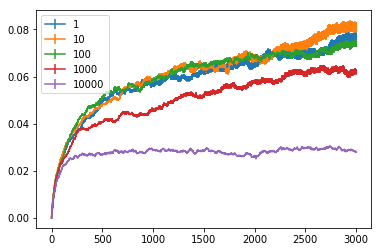
\includegraphics[scale=0.8]{Mean_plot_std.png}
\end{figure}

The standard deviation bars were 

\begin{figure}[hbt!]
    \centering
    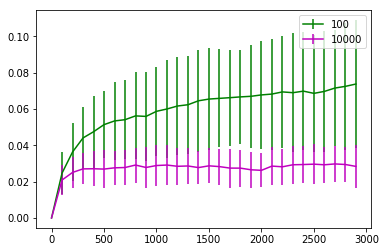
\includegraphics[scale=0.8]{Std_every100.png}
\end{figure}

\textsc{Starting weight trajectory different from true weights}
It is also interesting to see how well the algorithm manages to find the actual weights when the iterations begins from somewhere else. Now the initial guess for the MCMC iterations is set to be a random walk around 1.

\begin{figure}[hbt!]
    \centering
    \includegraphics[scale=0.8]{Start_it_1000.png}
\end{figure}


\begin{figure}[hbt!]
    \centering
    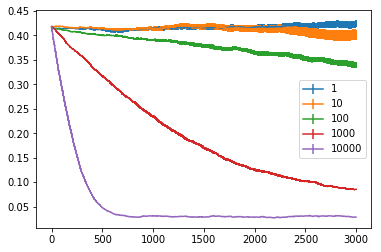
\includegraphics[scale=0.8]{MSE_starting_away.png}
\end{figure}

Figure \ref{w_trajectory_1000} and  shows how the weight trajectory develops over the iterations for 100 and 1000  (Note to myself: appendix? Since these are weight trajectories for single iterations their look is quite random. Maybe change to average weight trajectory of 100 or something?)

\begin{figure}[hbt!]
    \centering
    \includegraphics[scale=0.3]{fig/Start_it_1000.png}
    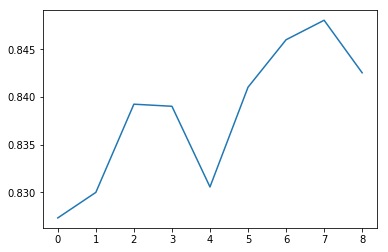
\includegraphics[scale = 0.3]{fig/1000_it_1000.png}
    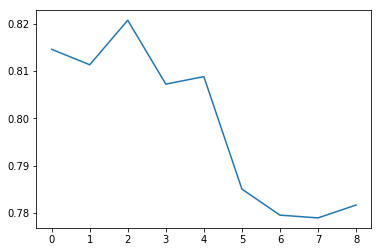
\includegraphics[scale = 0.3]{fig/2000_it_1000.png}\\
    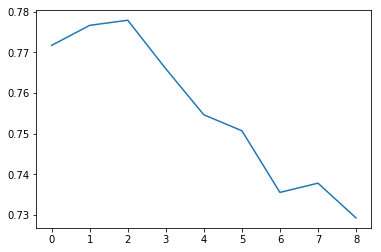
\includegraphics[scale = 0.3]{fig/3000_it_1000.png}
    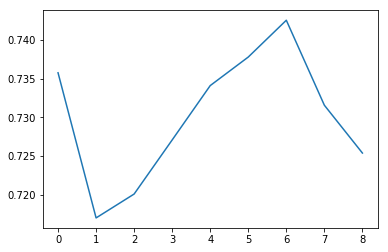
\includegraphics[scale = 0.3]{fig/4000_it_1000.png}
    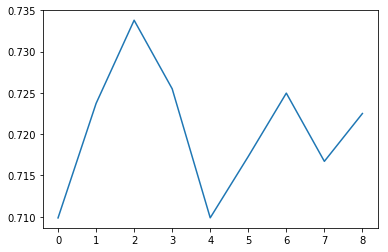
\includegraphics[scale = 0.3]{fig/5000_it_1000.png}
    \caption{Development of weight trajectory over iterations for 1000 trials. 0, 1000, 2000, 3000, 4000 and 5000 iterations}
    \label{w_trajectory_1000}
\end{figure}

\begin{figure}[hbt!]
    \centering
    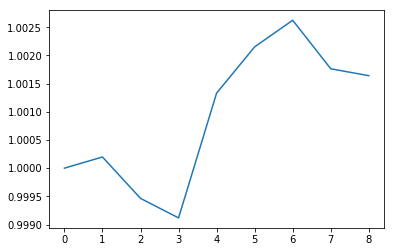
\includegraphics[scale=0.3]{fig/Start_it_100.png}
    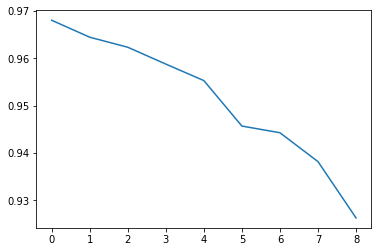
\includegraphics[scale = 0.3]{fig/1000_it_100.png}
    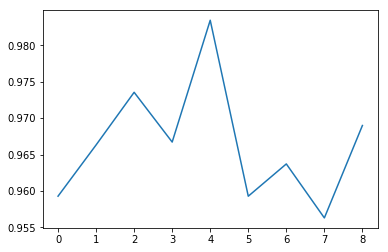
\includegraphics[scale = 0.3]{fig/2000_it_100.png}\\
    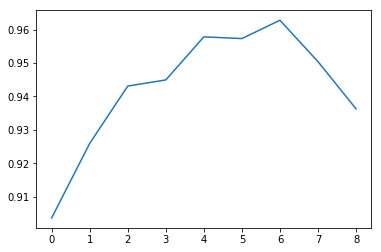
\includegraphics[scale = 0.3]{fig/3000_it_100.png}
    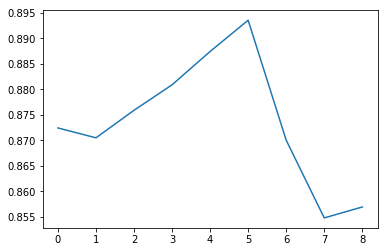
\includegraphics[scale = 0.3]{fig/4000_it_100.png}
    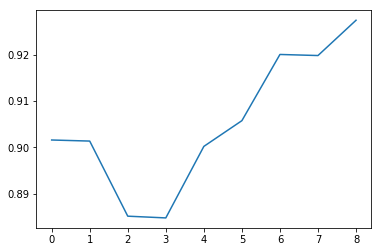
\includegraphics[scale = 0.3]{fig/5000_it_100.png}
    \caption{Development of weight trajectory over iterations for 100 trials. 0, 1000, 2000, 3000, 4000 and 5000 iterations}
    \label{w_trajectory_1000}
\end{figure}

\subsection{Weights generated by learning rule}

\begin{itemize}
    \item Describe test case and how I generated the weights
    \item Figures with results. Trying different variances for the prior ect
\end{itemize}

\begin{figure}[hbt!]
    \centering
    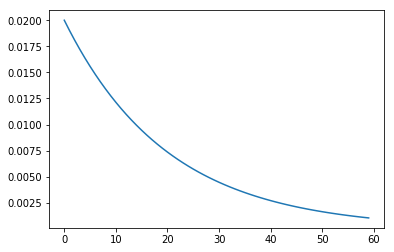
\includegraphics[scale=0.8]{Learning_rule.png}
\end{figure}

\cleardoublepage